\chapter{Introduction}

\minitoc%

Since the discovery of galaxies as distant objects from the Milky Way
\citep{Hubble+29}, many work has been done to understand how they formed and
what drives their observable properties (morphologies, color\ldots) at our
epoch and earlier in their evolution \citep{Benson+10,Silk+12,Silk+13}. The
combination of the structure formation of cold dark matter (CDM) particles
and their history \citep{Zentner+07}, with the baryon physics inside dark
matter halos \citep{Kravtsov+12} has been quite successful in reproducing
and explaining the observations from galaxy surveys. But there are still
some lacks in the galaxy formation scenario, which are headaches to solve
for theorists \citep{Weinmann+12}. A frequent solution to resolve this
puzzle is to introduce different recipes in galaxy formation simulations to
account for the missing physics that can reduce these discrepancies.
%
Such an example (and the most known problem of $\rm \Lambda$CDM) is the
overabundance of dwarf galaxies predicted by semi-analytical models (SAM) in
simulation of galaxy formation. Reducing their number implies to eject the
excessive baryons through several physical processes (feedback,
\citet{Brooks+13}) in order to make the dwarfs not resolvable. Such typical
processes are, for example, supernovae winds \citep{Hirschmann+13} or ram
pressure stripping. But introducing them leads to a more and more
complex scenario, and doesn't allow to clearly distinguish the effect of
each physical process on the galaxy evolution.

The galaxy formation is tightly correlated to the galaxy environment.
Indeed, galaxies are gregarious, leaving in different hosts environments
from isolated galaxies, to pairs, groups and clusters. This environment
impacts on galaxy properties in different manner, at different epochs,
through a large range of possible physical processes. But not all them are
important according to the redshift and environment of galaxies. The
characterization of the major physical process at work inside environments
should improve the predictions of SAM, by including more precise models and
recipes in the code, directly extracted from the analysis of the
observations. Moreover, this should also improve the galaxy formation
scenario constructed until now, and work as a test for this scenario. This
goal can only be achieved by an optimal definition of the galaxy
environment, in other words, an optimal selection of galaxy group and
clusters.

\section{Galaxy formation}
\label{sec:galaxy_formation}

The large structure of the Universe, observed in both sky and numerical
simulations, is in majority probed through galaxies and their content since the
dark matter only interacts gravitationally with the ``ordinary'' matter. This
is possible because galaxies formed inside these structures. At this time, the
commonly accepted scenario for the formation of large scale structure is the
hierarchical model, where small structures are created early in the story of
the Universe and then merged to become more massive. This is the $\Lambda$CDM
paradigm (CDM for cold dark matter) where the Universe is in expansion by
action of the dark energy and structures appear through the gravitational
interactions of cold dark matter, in opposition to hot dark matter where the
intrinsic velocities of dark matter avoid the formation of early small
structures. Inside these dark matter halos, the visible and non-dominant
fraction of the matter (baryons) follows the dark matter in its collapse, forms
a rotating disc, cooling and forming stars.

If this process goes without nothing to stop it, the mass of galaxies should
increases without limits: this is the overcooling problem \citep{White+78}. But
baryons are not only submitted to gravitation and several processes can prevent
the star formation inside such structures. At the two extremes of the halo mass
function, the gas is prevented from fragmenting into stars by heating
processes, avoiding the cooling of the gas to the center of the potential well
of dark matter structures. This heating can be intrinsic to the gas in the halo
because of the photo-ionization \citep{Rees+86} or due to a pre-heating of the
gas before it enters the halo \citep{Borgani+01}, acting essentially for low
mass halos. Supernova explosions have also a contribution to the re-heating of
the gas \citep{Dekel+86, Efstathiou+00} for low and intermediate masses. In
high masses halos, the cooling is less efficient but a large quantity of gas
can still cool to form very massive galaxies. Material ejected by active
galactic nuclei (AGN) is possibly an explanation for heating gas
\citep{Silk+98}, although the mechanism through which AGN operates is not well
understand. This is a consequence of the effect of the global environment of
galaxies onto their physical properties.
%
\begin{figure}[htb]
    \centering
    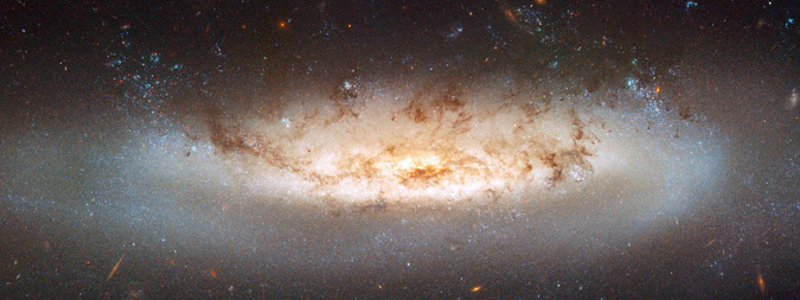
\includegraphics[width=\linewidth]{chapters/images/rampressure.jpg}
    \caption{An illustration of the ram pressure stripping experienced on a
    galaxy, whose interstellar gas in moved, quenching the star formation since
the ``fuel'' of this process is dropped out.\label{fig:rampressure}}
\end{figure}

The local environment plays also an important role. Several physical processes
are at work inside galaxy groups because of the galaxy over-density relatively
to the background field. They are mainly caused by interactions between each
galaxy and/or the group. Galaxy mergers (essentially major mergers involving
two galaxies of equivalent masses) are expected to morphologically transform
galaxies to spheroidal \citep{Naab+99,Bournaud+05}, and to create star
formation bursts inside merging galaxies \citep{Cox+08,Teyssier+10}. In the
other hand, the dense environment acts too on galaxy properties. Tidal forces
exerted by the group and the ram pressure stripping can remove the outer
gaseous regions in orbiting galaxies leading to a quenching of the star
formation \citep{Larson+80,Bekki+13}.

Some of these intra-group physics were already, more or less well, introduced
in SAM of galaxy formation \citep{Okamoto+03,Lanzoni+05,Font+08,Guo+11}. But
all these methods tend to over-simplify, by use of simple formulas, very
complex processes depending on several parameters and the galaxy environment. A
better modeling of the physics involved in galaxy group should improve the SAM
and correct their difficulties in fully describing the observed Universe. This
can only be achieved with a good definition of the environment for galaxies,
and galaxy groups in redshift space are exactly this definition of environment.

\section{The importance of galaxy groups}
\label{sec:the_importance_of_galaxy_groups}

\subsection{Galaxy group physics}
\label{sub:galaxy_group_physics}

Observed galaxy groups are a direct consequence of this hierarchical growth of
structure. Galaxies therein are affected by this growth since they formed in
dark matter sub-halos that merged with most massive halos along the Universe
expansion according to the hierarchical scenario \citep{Lacey+93}. So their
properties must be correlated with their parent dark matter halo and reflect
their physical processes history inside it. Some evidence of such a modulation
of galaxy properties were already observed previously on the galaxy luminosity
\citep{Robotham+10} and stellar mass \citep{Yang+09} functions, with the galaxy
environment.

Galaxies can be classified in two distinct populations: a blue population of
gas rich and young stellar population and a red one, poor in gas with an old
stellar population \citep{Driver+06}. This bi-modality is also visible in their
morphologies where red galaxies are essentially ellipsoidal and blue galaxies
are spiral. A segregation of these galaxies exists with the environment close
to our epoch (low redshifts): red galaxies lie in dense environment such as
clusters, while the blue population is more present in the field (outside dense
environments as clusters or groups). This is clearly an effect of the
environment, where in clusters, the dense region allows the intra-cluster gas
to be hot enough to stop the star formation of galaxies, leading to an old and
red stellar population. In lower dense region, mergers and various interactions
implying galaxies are frequent and boost the star formation.

But some other properties lead to discrepant results. For example, the specific
star formation rate (SSFR) doesn't show a dependence on the environment
according to~\cite{Peng+10} for high stellar mass galaxies, but following
\citet{vonderLinden+10}, there is clearly a trend of decline of the SSFR for
star forming galaxies towards groups center (for all galaxy masses). The
results of~\cite{Peng+10} are surprising since in groups and clusters, galaxies
are massive (in stars) due to the cannibalism that contributed in the past to
the formation of the structure. Moreover, the dense environment should quench
the star formation in galaxies due to the intra-cluster gas preventing the
formation of cold clouds, and so varying with the distance to the center of the
group. This contradiction is possibly explained by the selection of a tracer
for the environment in~\cite{Peng+10} that doesn't distinguish between the two
kind of environment: the local one related to the position of the galaxy
relatively to its halo, and the global environment that characterizes the total
mass embedded in the parent halo of the galaxy.
%
\begin{figure}[htb]
    \centering
    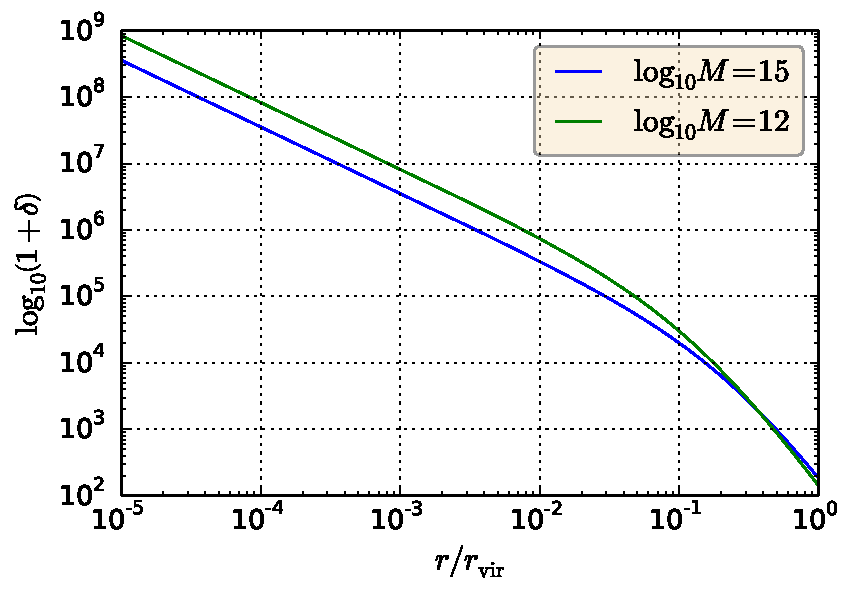
\includegraphics[width=0.6\linewidth]{figures/introduction/overdensity.pdf}
    \caption{The over-density relatively to the mean density for two different
        halos of mass $10^{12}$ and $10^{15} h^{-1} M_\odot$ in function of the
        distance to the halo center in units of virial radius $r_\mathrm{vir}$.
        A density profile from \citet{NFW+97} is assumed with concentrations
    computed from \citet{Maccio+08}.\label{fig:overdensity}}
\end{figure}
%
An example is shown in \bartreffigure{overdensity} where we plot the
over-density as defined in \citet{Peng+10} for two different halo masses with a
density profile from \citet{NFW+97} (see \bartrefappendix{profiles}), a
concentration from \citet{Maccio+08}, in function of the position relatively to
the halo center in units of virial radius. We chose two extremes masses
($10^{12}$ and $10^{15} h^{-1} M_\odot$) to have two very distinct halos. The
over-density is essentially sensitive to the local environment, but the global
one has only a small effect through the concentration parameter. With this
tracer, we can't observe a modulation of the SSFR\@, while the galaxy formation
scenario let us expect an influence of the halo mass with physical processes
regulating the star formation.
%
\remark{%
    Assuming the density profile of \citet{NFW+97}, the over-density $\delta$
    is:
    %
    \begin{equation}
        \delta = \cfrac{\rho \left(r\right) - \rho_m}{\rho_m}
    \end{equation}
    %
    Using equations from \bartrefappendix{profiles}, and writing the mean
    density of the Universe as $\rho_m=\Omega_m \rho_c$ where $\Omega_m$ is the
    density fraction of matter in the Universe (\citet{PlanckXVI} cosmology)
    and $\rho_c$ is the critical density equal to $3 H_0^2/ \left(8\pi
    G\right)$, we finally have:
    %
    \begin{equation}
    \delta = \cfrac{\Delta \overline\rho \left(r/r_\mathrm{vir}\right)}
    {3\Omega_m} - 1
    \end{equation}
    %
    with $\Delta$ the value of the density in units of the critical density
    used to defined a halo relatively to the background, and $\overline\rho$
    the normalized density profile as defined in
    \bartrefappendix{profiles}.
}

Moreover, a clean characterization of the environment from the redshift space
is difficult since the redshift distortions \citep{Jackson+72}, called also
Fingers-of-God \citep{Tully+78}, caused by the velocity dispersion of the
galaxy group can create overlapping between galaxies of foreground or
background groups. But the over-density used in \citet{Peng+10} is computed
from the nearest neighbors of each galaxies, clearly affected by interlopers
because of projection effects.

\subsection{Galaxy groups as tests}
\label{sub:galaxy_groups_as_tests}

Galaxy groups are not just limited to test and improve the models for the
galaxy formation theory, but also appear in other astrophysical domains. In
cosmology, they are a tool to access the cosmological parameters, such as
the dark energy fraction \citep{Wang+98}. General relativity can be tested
with them \citep{Wojtak+11}. \com{and so many other examples\ldots}

\section{Characterizing environment}
\label{sec:characterizing_environment}

\subsection{History}
\label{sub:history}

Many galaxy group catalogs were already published, usually following the first
publications of data from galaxy surveys. First attempts were done with human
selections \citep{Abell+58,Zwicky+61,Rose+76}. The selection was based on non
physical assumptions on galaxy groups, with certain criteria for a visual
over-density of galaxies.

Then the percolation or Friends-of-Friends (FoF) algorithm followed, based on
the knowledge of galaxy physics at this epoch \citep{Huchra+82,Nolthenius+87}.
One of its advantages is that it is based on a physical choice for the way to
link galaxies between them in groups. A linking length is used to relate to
galaxies that are closer than this distance in redshift space. This needs the
use of two different linking lengths in the line-of-sight and perpendicular
directions to avoid the redshift distortions effect. But as argued in
\citet{Duarte+14}, with some priors in the galaxy distribution, these links must
be adjusted to the mass of the group (i.e.\ its richness) to be complete in the
galaxy selection. More recently, \citet{Eke+04} and \citet{Berlind+06}
published too galaxy groups catalogs from the application of the percolation
algorithm, but taking into account, in their selection, the incompleteness
induced by the galaxy surveys used.

\citet{Marinoni+02} developed a method similar to FoF but with the use of a
redshift space partitioned into Voronoi cells, to have an initial seed for the
over-density (Voronoi cells volume trace the galaxy density) around each
galaxy. But this method suffers from the necessity to use it in small surveys
in angle because of the difficulty to create a tessellation of the celestial
sphere directly.

With the increasing advances in the galaxy formation processes, capacities of
numerical computation and predictions of the cosmological simulations, started
to appear Bayesian algorithms that used priors on galaxy groups to improve
their extraction from galaxy surveys. \citet{Yang+05,Yang+07} developed an
iterative method to select galaxy groups based on a density contrast criterion,
which uses assumptions based on cosmological simulation results for the density
profile of groups.

Galaxy surveys have limitations that are difficult to overcome in galaxy group
algorithms. In the case of photometric redshifts surveys, probabilistic
Friends-of-Friends were developed to attempt avoiding the large (and sometimes
catastrophic) uncertainties in redshift measures \citep{Liu+08}. Then,
probability was used to improve the membership of galaxies inside their groups,
as \citet{DominguezRomero+12}, allowing a more flexible way to affect galaxies.

Finally, group finding algorithms continue their insertion of galaxy formation
results, combining it with the advantage of geometrical methods. An example is
\citet{MunozCuartas+12} that used a FoF applied on dark matter halos associated
to galaxies, with the initial assumption that all galaxies are their own halo,
and so the central galaxy mass is a tracer of the density field (the most
massive central galaxies are associated to the most massive halos).

\subsection{And now\ldots?}
\label{sub:and_now}

Actual and next generations of galaxy surveys allow us to probe galaxy groups
in different aspects, each of them with their improvements and limits. Sloan
Digital Sky Survey (SDSS), with its around one million of spectroscoped
galaxies, gives us a good overview of the density field for a large range of
redshifts. But this abundance of precise redshifts as the counterpart that not
all galaxies have spectroscopic redshifts, and around 5--10\% of galaxies,
because of the fiber collision problem \citep{Blanton+03}, need to fall back to
photometric redshifts, more inaccurate. The Galaxy And Mass Assembly, at its
final stage, will contain around $300\;000$ galaxies with a spectroscopic
redshift \citep{Hopkins+13}, less than the SDSS\@. But the completeness of the
sample will be higher than the SDSS with $\simeq99\%$ of the sample
spectroscoped. The counterpart is a less precise measurement of galaxies
recession velocities \citep{Robotham+11,Hopkins+13}. Moreover, the adjoining
angular size is lower because of the fragmentation of the survey regions. But
those galaxy samples are from different sky region allowing to take into
account the cosmic variance in the statistics. In consequence, galaxy group
algorithms must be flexible to be applied and give the same result in many,
different and (surprisingly) creative future galaxy survey projects. Their
common limitations and advantages must be take into account when developing it.

Galaxy group algorithms give different results, maybe caused by a lack of
interlopers removal and/or bad completeness. Difficult to estimate since tested
in differently constructed mock catalogs. \com{Need to really check that!}

So we need to go beyond the usual standard and static definition of groups and
work with the inevitable polluted environment of extracted galaxy groups to
have a precise understanding of the major physical processes at work inside
galaxy groups. We start by an overview of some common grouping algorithms,
their innovations and limitations in \bartrefchapter{galaxy_group_algorithms}.
Since such algorithms must be tested in order to access their capacities in
recovering the clustering from redshift space, we detailed the construction of
a galaxy mock catalogue, difficulties inherent to its creation and biases
introduced voluntary or not inside \bartrefchapter{mock}. We were also
interested in the most popular algorithm that is the Friends-of-Friends or
percolation algorithm and performed a detailed test on its performances in
\bartrefchapter{friends_of_friends_algorithm}. MAGGIE, a probabilistic galaxy
group algorithm that avoids the importance of interlopers in the galaxy group
properties observed is described and analyzed in \bartrefchapter{MAGGIE}. In
\bartrefchapter{sdss}, we described our analysis of the Sloan Digital Sky
Survey in the goal of a future application of MAGGIE on its database.

% vim: set tw=79 :
